\section{Reading x86-64 Assembly}

\begin{frame}[plain,noframenumbering]
    \centering
    \scalebox{3}{Reading x86-64 Assembly}

    \scalebox{2}{\ldots for fun and profit}
\end{frame}

\begin{frame}[fragile]{Function Prologue \& Epilogue}
    \begin{itemize}
        \item Few lines of code at the beginning (\textit{prologue}) and end (\textit{epilogue}) of a function, which \textbf{prepares} (and eventually restores)
        \begin{itemize}
            \item the \textbf{stack} and 
            \item \textbf{registers}
        \end{itemize}
        \item Not part of assembly: \textbf{convention} (defined \& interpreted differently by different OS and compilers)
    \end{itemize}

    \begin{columns}[t]
        \begin{column}{.45\textwidth}
            \textbf{Prologue}
            \begin{lstlisting}[language={}]
push rbp     ; rbp: frame pointer
mov rbp, rsp ; rsp: stack pointer
sub rsp, N
            \end{lstlisting}
            alternatively
            \begin{lstlisting}[language={}]
enter N, 0
            \end{lstlisting}
            (reserve \texttt{N} bytes on stack for local use)
        \end{column}
        \begin{column}{.45\textwidth}
            \textbf{Epilogue}
            \begin{lstlisting}[language={}]
mov rsp, rbp
pop rbp
ret
            \end{lstlisting}
            alternatively
            \begin{lstlisting}[language={}]
leave
ret
            \end{lstlisting}
        \end{column}
    \end{columns}
\end{frame}

\begin{frame}[fragile]{Stack frame for function call}
    \begin{columns}
        \begin{column}{.4\textwidth}
            \begin{itemize}
                \item \texttt{CALL} = \texttt{PUSH} \textit{address of next instruction} + \texttt{JMP} \textit{target}
                \item \texttt{RET} pops return address and transfers control there
                \item pass arguments 1 \ldots 6 in registers (\texttt{rsi}, \texttt{rdx}, \ldots)
            \end{itemize}
        \end{column}
        \begin{column}{.6\textwidth}
            \begin{Verbatim}
┌──────────────┐
│ ...          │
│ 8th Argument │ (rbp + 24)
│ 7th Argument │ (rbp + 16)
├──────────────┤
│ rip          │ (return address)
│ rbp          │ (rbp)
├──────────────┤
│ rbx          │
│ r12          │
│ r13          │ (rsp)
└──────────────┘
            \end{Verbatim}
            (stack frame for function call with 8 arguments and local registers \texttt{rbx}, \texttt{r12} and \texttt{r13})
        \end{column}
    \end{columns}
\end{frame}

\begin{frame}[fragile]{Reading assembly for fun and profit}
    \begin{columns}[t]
        \begin{column}{.45\textwidth}
            \inputcpplisting{snippet2}
        \end{column}
        \begin{column}{.45\textwidth}
            \inputasmlisting{snippet2}
        \end{column}
    \end{columns}
\end{frame}

\begin{frame}[fragile]{Reading assembly for fun and profit}
    \begin{columns}[t]
        \begin{column}{.45\textwidth}
            \inputcpplisting{snippet3}
        \end{column}
        \begin{column}{.45\textwidth}
            \inputasmlisting{snippet3}
        \end{column}
    \end{columns}
\end{frame}

\begin{frame}[fragile]{Reading assembly for fun and profit}
    \begin{columns}[t]
        \begin{column}{.45\textwidth}
            \inputcpplisting{snippet4}
        \end{column}
        \begin{column}{.45\textwidth}
            \inputasmlisting{snippet4}
        \end{column}
    \end{columns}
\end{frame}

\begin{frame}[fragile]{Name mangling: \texttt{C++} vs \texttt{C}}
    \begin{columns}[t]
        \begin{column}{.45\textwidth}
            \inputcpplisting{snippet1}

% REMOVE_FOR_PRINT {
            \only<2>{%
% REMOVE_FOR_PRINT }
                \textbf{Why?}
                \begin{itemize}
                    \item overloading
                    \item namespaces
                    \item templating
                \end{itemize}
                (Name of function doesn't suffice to resolve \texttt{JMP} location)%
% REMOVE_FOR_PRINT {
            }
% REMOVE_FOR_PRINT }
        \end{column}
        \begin{column}{.45\textwidth}
            \inputasmlisting{snippet1}
        \end{column}
    \end{columns}
\end{frame}

\begin{frame}[fragile]{Name mangling in \texttt{C++}}
    \begin{columns}[t]
        \begin{column}{.45\textwidth}
            \inputcpplisting{snippet5}
        \end{column}
        \begin{column}{.45\textwidth}
            \inputasmlisting{snippet5}
        \end{column}
    \end{columns}

    \begin{itemize}
        \item \texttt{C++} does not standardize name mangling
        \item \textit{Annotated C++ Reference Manual} even actively discourages usage of common mangling schemes. (Prevent linking when other aspects of ABI are incompatible.) 
    \end{itemize}
\end{frame}

\section{What is ABI?}

\begin{frame}[plain,noframenumbering]
    \centering
    \scalebox{3}{What is ABI?}
\end{frame}

\begin{frame}{What is ABI (\textit{\textbf{A}pplication \textbf{B}inary \textbf{I}nterface})?}
    \begin{columns}
        \begin{column}{.6\textwidth}
            \textbf{Specifies interaction of functions and types across TUs${}^{\color{vertexDarkRed}\dagger}$ (translation units)}
            \only<1>{%
            \begin{itemize}
                \item Platform-specific (\textit{e.g.}, Linux on x86-64 CPU)
                \item Vendor-specified (\textit{e.g.}, gcc)
                \item not controlled by \href{http://www.open-std.org/jtc1/sc22/wg21/}{WG21}
            \end{itemize}}
            \only<2>{%
            covering:
            \begin{itemize}
                \item Name mangling of functions
                \item Name mangling of types
                \item \texttt{sizeof} and alignment of objects
                \item Bytes semantics of the binary representation of objects
                \item Calling convention
            \end{itemize}}
            (Titus Winters: \textit{Similar to a binary network protocol})
        \end{column}
        \begin{column}{.3\textwidth}
            \centering
            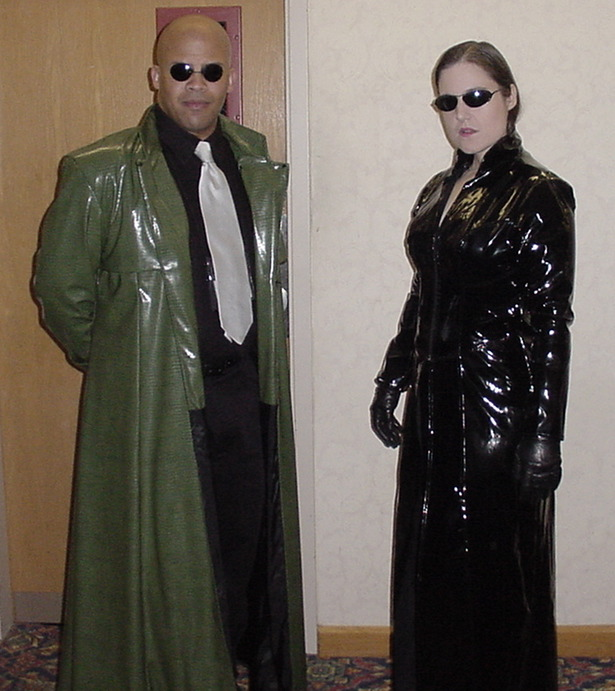
\includegraphics[height=.6\textheight]{matrix.png}\\
            {\footnotesize \href{https://commons.wikimedia.org/wiki/File:Spencerian_Matrix_cosplay.jpg}{Photo by Spencerian at \texttt{en.wikipedia.org} (2005)}}
        \end{column}
    \end{columns}

    \vspace{5mm}

    \footnotesize ${}^{\color{vertexDarkRed}\dagger}$ \textit{TU}: ultimate input to the compiler from which an object file is generated (\textit{i.e.}, typically the \texttt{.cpp} file)
\end{frame}

\begin{frame}[plain,noframenumbering]
    \centering
    \scalebox{3}{Why should I care?}

    \scalebox{1.2}{\ldots do you depend on any pre-compiled shared library?}
\end{frame}

\begin{frame}{Why should I care?}
    \textbf{Why should I care?}
    \begin{itemize}
        \item \textbf{Linking} different TUs requires usage of same ABI
        \item Typically a problem at API boundaries when combining TUs (\textit{e.g.}, shared libraries) that were compiled at different \textbf{time}s
        \item Similar to binary network protocols: ABI tells you how to interpret bytes
    \end{itemize}

    \vspace{5mm}

    \centering
    \scalebox{1.2}{Why should I care? $\Leftrightarrow$ Why do network protocols have versions?}

    \vspace{5mm}
    (Problem: not all ABIs encode version number)
\end{frame}

\begin{frame}{ABI: the problem}
    \centering
    \textbf{ABI does not encode version number}
    \begin{itemize}
        \item \textbf{Q}: How to check if a given TU uses a compatible ABI?
        \item \textbf{A}: You can't!
        \item What happens if ABI is incompatible?
        \begin{itemize}
            \item[(a)] Linking fails during compile time (good)
            \item[(b)] Program spectacularly dies during run time (bad)
        \end{itemize}
        \item Why isn't this a common problem?
        \begin{itemize}
            \item Itanium ABI is mostly stable since \texttt{C++11}
        \end{itemize}
    \end{itemize}
\end{frame}

% REMOVE_FOR_PRINT {
\addtocounter{framenumber}{-1}
\begin{frame}[plain,noframenumbering]
    \centering
    
\includegraphics[width=.9\textwidth]{history.png}
\end{frame}
% REMOVE_FOR_PRINT }

\begin{frame}{ABI breakage of \texttt{std::string}}
    \begin{columns}
        \begin{column}{.55\textwidth}
            \begin{itemize}
                \item Before \texttt{C++11}: libstdc++ relied on copy-on-write (COW)
                \item \texttt{C++11} disallows COW 
                \begin{itemize}
                    \item fewer indirections
                    \item short string optimization (SSO)
                \end{itemize}
                \item Problem: passing COW string to impl that expects SSO \textbf{may link} (same mangled name)!
                \begin{itemize}
                    \item one (quad-)word passed
                    \item three (quad-)words read
                \end{itemize}
                \item \textit{Solution}${}^{\color{vertexDarkRed}\dagger}$: gcc changed mangled name
            \end{itemize}
        \end{column}
        \begin{column}{.35\textwidth}
            \inputcpplisting{snippet6}
        \end{column}
    \end{columns}

    \vspace{3mm}

    \scalebox{1.2}{$\hookrightarrow$ Take-away for compiler vendors: ABI break was a huge disaster}

    \vspace{3mm}

    \footnotesize ${}^{\color{vertexDarkRed}\dagger}$ RHEL\,7 still uses old \texttt{std::string} ABI to provide compatibility for older \texttt{.so}
\end{frame}
